\documentclass{sigchi}

% Remove or comment out these two lines for final version
\toappearbox{\Large Submitted to CHI'13. \\Do not cite, do not circulate.}
\pagenumbering{arabic}% Arabic page numbers for submission. 

% Use \toappear{...} to override the default ACM copyright statement (e.g. for preprints).

% Load basic packages
\usepackage{balance}  % to better equalize the last page
\usepackage{graphics} % for EPS, load graphicx instead
\usepackage{times}    % comment if you want LaTeX's default font
\usepackage{url}      % llt: nicely formatted URLs
\usepackage{listings}
\usepackage{gensymb}
\usepackage{multirow}

%\usepackage{caption}
%\usepackage{subcaption}

% llt: Define a global style for URLs, rather that the default one
\makeatletter
\def\url@leostyle{%
  \@ifundefined{selectfont}{\def\UrlFont{\sf}}{\def\UrlFont{\small\bf\ttfamily}}}
\makeatother
\urlstyle{leo}


% To make various LaTeX processors do the right thing with page size.
\def\pprw{8.5in}
\def\pprh{11in}
\special{papersize=\pprw,\pprh}
\setlength{\paperwidth}{\pprw}
\setlength{\paperheight}{\pprh}
\setlength{\pdfpagewidth}{\pprw}
\setlength{\pdfpageheight}{\pprh}


% create a shortcut to typeset table headings
\newcommand\tabhead[1]{\small\textbf{#1}}


%************* Andreas Additions
\newcommand{\squishlist}{
 \begin{list}{$\bullet$}
 {
  \setlength{\itemsep}{0pt}
  \setlength{\parsep}{3pt}
  \setlength{\topsep}{3pt}
  \setlength{\partopsep}{0pt}
  \setlength{\leftmargin}{1.5em}
  \setlength{\labelwidth}{1em}
  \setlength{\labelsep}{0.5em} } }

\newcommand{\squishend}{
  \end{list}  }

% Alter some LaTeX defaults for better treatment of figures:
    % See p.105 of "TeX Unbound" for suggested values.
    % See pp. 199-200 of Lamport's "LaTeX" book for details.
    %   General parameterbnos, for ALL pages:
    \renewcommand{\topfraction}{0.9}	% max fraction of floats at top
    \renewcommand{\bottomfraction}{0.8}	% max fraction of floats at bottom
    %   Parameters for TEXT pages (not float pages):
    \setcounter{topnumber}{2}
    \setcounter{bottomnumber}{2}
    \setcounter{totalnumber}{4}     % 2 may work better
    \setcounter{dbltopnumber}{2}    % for 2-column pages
    \renewcommand{\dbltopfraction}{0.9}	% fit big float above 2-col. text
    \renewcommand{\textfraction}{0.07}	% allow minimal text w. figs
    %   Parameters for FLOAT pages (not text pages):
    \renewcommand{\floatpagefraction}{0.7}	% require fuller float pages
	% N.B.: floatpagefraction MUST be less than topfraction !!
    \renewcommand{\dblfloatpagefraction}{0.7}	% require fuller float pages

	% remember to use [htp] or [htpb] for placement


% Adds a space between the text and the [T]op \hline
% Must use the \T *within* a cell, not right after the \hline
\newcommand\T{\rule{0pt}{2.5ex}}%{3.1ex}}

% Adds a space between the text and the [B]ottom \hline
% Must use the \B *within* a cell, not right after the \hline
\newcommand\B{\rule[-1ex]{0pt}{0pt}}%[-1.7ex]{0pt}{0pt}}

% To get the \url{} command that allows line breaks in URLs,
% directory paths, etc:


%************* End Andreas Additions


% Make sure hyperref comes last of your loaded packages, 
% to give it a fighting chance of not being over-written, 
% since its job is to redefine many LaTeX commands.
\usepackage[pdftex]{hyperref}
\hypersetup{
pdftitle={SIGCHI Conference Proceedings Format},
pdfauthor={LaTeX},
pdfkeywords={SIGCHI, proceedings, archival format},
bookmarksnumbered,
pdfstartview={FitH},
colorlinks,
citecolor=black,
filecolor=black,
linkcolor=black,
urlcolor=black,
breaklinks=true,
}


% End of preamble. Here it comes the document.
\begin{document}

\title{Programming Robots at the Museum}

% Note that submissions are blind, so author information should be omitted


%\numberofauthors{2}
%\author{
%  \alignauthor Andreas Paepcke\\
%    \affaddr{Stanford University}\\
%    \affaddr{Stanford, CA}\\
%    \email{paepcke@cs.stanford.edu}
%  \alignauthor Caroline Pantofaru, Dirk Thomas, Austin Hendrix, Sarah Elliot, Sharon Marzouk\\
%    \affaddr{Willow Garage}\\
%    \affaddr{Menlo Park, CA}\\
%    \email{\{pantofaru,dthomas,ahendrix,selliott,smarzouk\}@willowgarage.com}
%    }

% \author{
%  \parbox[t]{18.0cm}{\centering 
%    {\em Andreas Paepcke\**}, 
%    {\em Caroline Pantofaru\**\**}, 
%    {\em Dirk Thomas\**\**}, 
%    {\em Austin Hendrix\**\**}, 
%    {\em Sharon Marzouk\**\**},
%    {\em Sarah Elliot\**\**}}\\
%  \\
%  \parbox[t]{5.0cm}{\centering
%         \**Stanford University\\
%         353 Serra Mall\\
%         Stanford, CA 94305\\
% 	paepcke@cs.stanford.edu}\\
%  \\
%  \parbox[t]{10.0cm}{\centering
%     	\**\**Willow Garage\\
% 	68 Willow Road\\
% 	Menlo Park, CA 94025\\
%        \{pantofaru,dthomas,ahendrix,smarzouk,selliott@willowgarage.com\}}
% }

% Teaser figure can go here
%\teaser{
%  \centering
%  \includegraphics{Figure1}
%  \caption{Teaser Image}
%  \label{fig:teaser}
%}

\maketitle

\begin{abstract}
  \end{abstract}

\keywords{assistive technology; prolonged engagement; collaborative conversation; story telling game}

\category{H.5.2}{Information Interfaces And Presentation}{User Interfaces - Interaction styles}

\terms{Human Factors; Design}


\tolerance=400

% Macros for the Python and Puppet interface names.
% Using these in case we want to change these terms:
\newcommand{\py}{{\em coding interface}}
\newcommand{\puppet}{{\em Puppet interface}}
\newcommand{\semi}{{\em semi-autonomous interface}}
\newcommand{\tapper}{{\em Tapper}}

%\newcommand{\degree}{$^\circ$}


\section{Introduction}

%*****
% Note: use macros \py, \semi\, and \puppet as the names for the three
% interfaces: Python, original IK based puppet design, and ultimate
% design used in the museum.
%
%o hack the future: number of hours
%o number of hours for exhibit open
%o three versions: Programming (\py), old (\semi), and Puppet (\puppet)
%*****

\section{Introduction}
We collaborate with a motion and speech impaired individual, Henry,
who enjoys conversing. The speech impairment is complete. Quadriplegia
while severely limiting, does allow Henry to move his head in
affirmation or negation. His hand can operate a mouse button. One of
his communication modes is via a text-to-speech system ({\em tts}). A
camera mounted on top of his laptop tracks a confetti sized white dot
pasted on the lower left of his glasses. The resulting cursor control
allow Henry to hunt down the keys of an onscreen keyboard. On a very
good day the resulting speed is 15 words per minute. The tts produces
sound once a sentence is complete. Uttering words as Henry types them
would work, but this approach makes it difficult for listeners to
track the very slowly evolving sentences in their minds. Poor
tts performance for some words would additionally impede
comprehension, which is supported by context when a full sentence is
pronounced in a flow. 

This slow communication channel results in very frustrating
experiences during gatherings like parties. A guest will make a remark
to Henry, who will go to work on an answer. To the conversation
partner Henry looks frozen, peering at his laptop screen whose back
surface reveals nothing to the expectant partner. Often the potential
conversation partner wanders off bewildered before Henry can finish
his response sentence.

One improvement would be to install a second display on the backside
of Henry's laptop. Inexpensive, USB based options are available. This
option would at least allow a listener to understand that information
is forthcoming. The option does not help as much as possible in
keeping the listener(s) actively involved in the conversation. 

In an attempt to ameliorate the situation further we developed
EchoTree. EchoTree is a distributed, collaborative word
tree. Figure~\ref{fig:echoTree} shows an example.
\begin{figure}
   \centering
   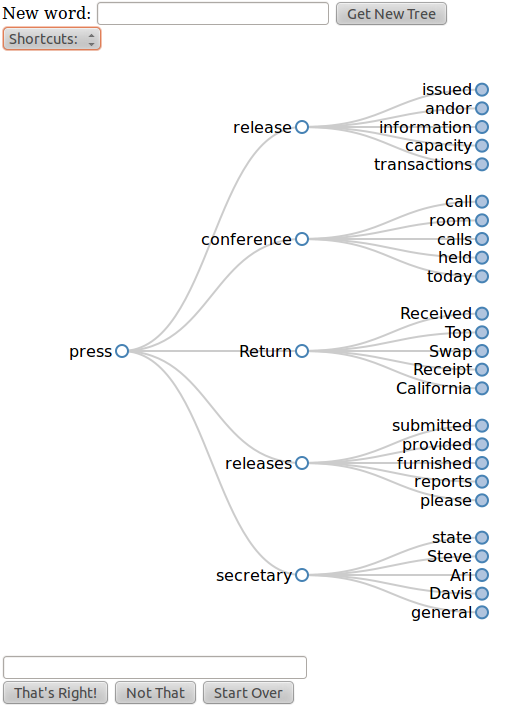
\includegraphics[width=0.6\columnwidth]{Figs/echoTreeScreenshot.png}
   \caption{Screenshot of an EchoTree browser.}
   \label{fig:echoTree}
\end{figure}

\section{User Experience}

EchoTrees are browser applications that can be viewed anywhere, by
multiple users. For example, the secondary display facing a
conversation partner in the option discussed earlier could show an
EchoTree. Alternatively, a conversation partner's smartphone could
{\em tune in} to Henry's EchoTree. After describing the interface and
some of its interaction affordances we explain how an EchoTree can be
related to Henry's response activity.

The word on the left most node of Figure~\ref{fig:echoTree} is called
the {\em root word}, in case of the Figure the root word is {\em
  press}. Links connect the root node to the five `most frequently
following' other words.  `Most frequently following' is measured in
the context of an underlying text collection. We will discuss this
dependency later.

Each of the word followers is connected to the five words that most
frequently follow {\em it} in the underlying texts. Following, for
example, the top branches in Figure~\ref{fig:echoTree} we find the
sequence ${press, release, issued}$.

In the current implementation anyone viewing an EchoTree on their
device may click or tap on one of the circles. In response all the
displayed EchoTrees are {\em re-rooted}: the selected word becomes the
root of a new tree. All follow words are recomputed, and a new tree is
displayed on all browsers. Figure~\ref{fig:todayTree} shows the result
of clicking on the word {\em today} in Figure~\ref{fig:echoTree}'s
tree. 
\begin{figure}
   \centering
   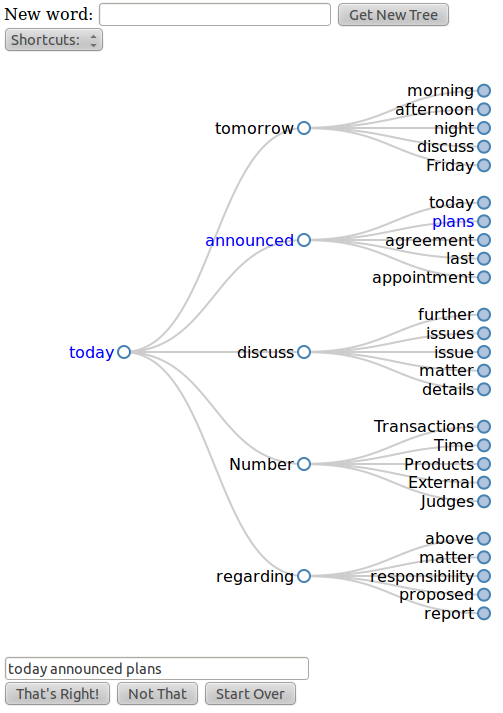
\includegraphics[width=0.6\columnwidth]{Figs/echoTreeRootToday.png}
   \caption{EchoTree re-rooted in `today'. Blue words were user
     selected, adding them to the sentence box.}
   \label{fig:todayTree}
\end{figure}
Alternatively, one may type a new word into the text box at the top,
and click on the button {\em Get New Tree}. This action again creates
a new tree, rooted at the new word, and displayed everywhere.

Instead of clicking/tapping on a circle, one may target one of the
words with a click or tap. This action causes two changes in the
display. First, the targeted word turns blue, and second, the word is
added to the text field at the bottom of the display. This field is
called the {\em sentence box}. Figure~\ref{fig:todayTree} shows the
result of clicking on {\em today}, then {\em announced}, and finally
{\em plans}.

The EchoTree facility can be used for a number of purposes. In the
context of Henry interacting in a conversation, the facility may be
used as follows. 

\subsection{Collaborative Conversing}

As Henry types words, EchoTrees in the browsers of all tuned in
listeners will evolve, the latest word always serving as root. Any
word that Henry completes is additionally appended to the sentence
box. Listeners, meanwhile may active think ahead and guess where Henry
might be headed. After scanning the current EchoTree they can call out
possibilities. If Henry hears a hit, he can click on the {\em That's
  Right} button, or nod. After a successful guess Henry can continue,
skipping one of more words.

Of course, if Henry notices a word that matches his intention, he can
click on that word in the EchoTree himself. If the content of the
sentence box is hopelessly wrong, the {\em Start Over} button will
clear the box, and turn off all blue (i.e. selected) words in the
EchoTree. 

The underlying machinery will not include a fixed set of stopwords in
the EchoTrees. This filtering helps maximize use of the limited screen
real-estate. Sometimes participants may wish to enrich sentences with
fill words. The pull-down menu below the {\em New word} field fills
that need (Figure~\ref{fig:shortcuts}). Selecting any of these words
will enter them in the sentence box. Again, in the current
implementation this addition appears in all views of the EchoTree. 
\begin{figure}
   \centering
   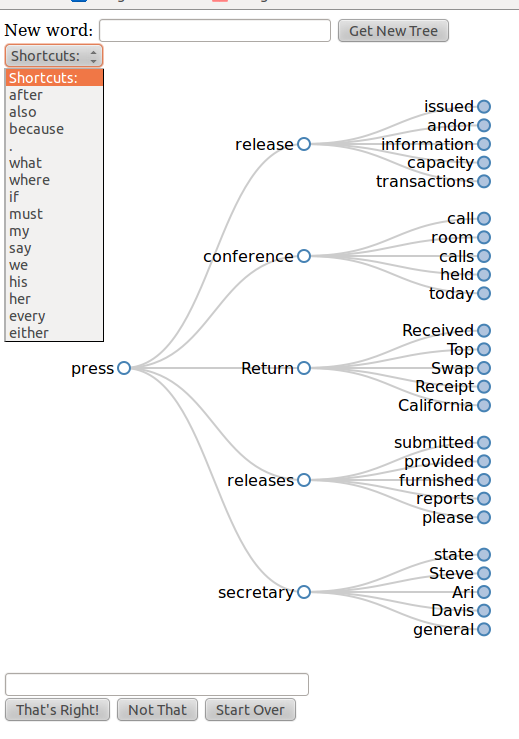
\includegraphics[width=0.5\columnwidth]{Figs/echoTreePulldownSnapshotSmall.png}
   \caption{Shortcut words are available as fillers for the sentence
     box. These stopwords will not occur in EchoTrees.}
   \label{fig:shortcuts}
\end{figure}
Note that the use of EchoTrees for collaborative conversation is not
limited to face-to-face situations, like parties. Communication
with Henry via the telephone are also an option. The remote
participant tunes into Henry's EchoTrees, and offers guesses over the
phone. Since Henry nodding assent is not an option in this scenario,
the {\em Not That} button can serve as a negative response.

\subsection{Story Telling Game}

Instead than supporting a directed conversational thread,
EchoTrees can serve as a collaborative story telling
facility. Geographically distributed players click on words in a
starting EchoTree, collaboratively adding words to the sentence
box. Various rules might govern the process. Participants might take
turns, or work at speed without sequence limitations. Re-rooting might
earn a demerit, while opening new possibilities. 

This application is accessible to disabled and non-impaired
participants. Again, the goal is mutual engagement. Appropriate rules
in this scenario can provide satisfying interaction even in the
presence of speed limitations.

\subsection{Architecture}

Figure~\ref{fig:arch} shows how the EchoTree system is
constructed. 
\begin{figure}
   \centering
   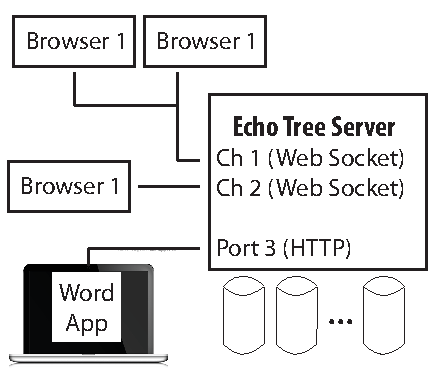
\includegraphics[width=0.5\columnwidth]{Figs/echoTreeArch.pdf}
   \caption{EchoTree architecture. Channels are implemented as
     WebSocket ports. Browsers tune in to different EchoTree channels.}
   \label{fig:arch}
\end{figure}
Central, or distributed EchoTree servers each manage some
number of distinct EchoTree channels. All facilities described above
operated on one channel. All shared EchoTree views are refreshed, and
request re-rooting on one channel. 

Multiple, unrelated EchoTree sequences may be served by a single
server, using different ports. In Figure~\ref{fig:arch}
Browers~1 is separated from Browsers two and three, which share all
EchoTree transmissions.

Browsers communicate with EchoTree servers via WebSocket connections,
which are bi-directional. This bidirectionality enables the re-rooting
requests from browsers back to the server.

Figure~\ref{fig:arch} also shows an HTTP port family. These
ports can push new words to the echo server, triggering the multicast
of a new EchoTree to all browsers on the respective channel. These
HTTP connections are simpler than the more versatile WebSocket
connections. They are provided for easy connection with word entry
support applications on Henry's machine. For example, Henry uses an
application that offers word completions as he types a word. The HTTP
method of pushing words to the EchoTree server can be attached to this
application. This method allows Henry to focus on typing in his usual
environment, and not being forced to interact with a browser's {\em
  New Word} entry to push a new word (and consequently new EchoTree).

Figure~\ref{fig:arch} shows a series of databases with word
pair frequencies that are the basis for the generation of the
trees. Each database holds lists triples: a word, a follower word, and
a frequency count. These {\em bigram} counts may originate from any
text collection. The trees of the above figures are based on bigrams
from the Enron collection ~\ref{enron}. In the following section we
examine some aspects of these underlying collections, which strongly
influence the induced EchoTrees.

\section{Effectiveness Experiment}

EchoTree could be effective along several dimensions. Each dimension
implies a different evaluation method:
\begin{enumerate}
\item Conversation acceleration through word prediction.
\item Conversation acceleration by conveying intent.
\item Encouragement through bi- or multilateral engagement.
\item Fun
\end{enumerate}
We measured the first item in an experiment, which we will describe in
this section. This dimension works by accurately predicting the next
word the current utterance originator is planning to type.

The second dimension in the above list contributes not through
prediction, but by helping the listener imagine indirectly where the
UO is heading. The inspiration might for example arise from
associations with words that occur in the EchoTree, though those word
not literally in the UO's plan.

The third dimension simply helps keep the conversation partners
connected. All listeners can at least observe progress, and maybe
anticipate a chance to complete a sentence soon.

The final dimension, finally, contributes by raising enjoyment in the
interaction. This element is most obvious in the story telling
scenario. All dimensions can contribute cumulatively, and are worthy
of evaluation. An examination of the word prediction power is an
important start. 

\subsection{Setup}
As with all word prediction, EchoTree's predictive power depends on
the match between the word source and the underlying frequency
data. We tested and compared four such pairings in a two-by-two
experiment, as shown in Table~\ref{tab:conditions}.

\begin{table}
    \begin{tabular}{|r|c|c|}
        \hline
        ~                & {\bf Enron Collection} & {\bf Google Bigrams} \\ \hline
        {\bf Henry}      & ~                & ~                    \\ 
        {\bf Enron EmpX} & ~                & ~                    \\
        \hline
    \end{tabular}
    \caption{Two-by-two experiment matching utterance originators with
      word prediction sources.}
    \label{tab:conditions}
\end{table}

\subsection{Results}
\section{Discussion}
\section{Related Work}
\section{Future Work}
\section{Conclusion}

%-------------------


% Balancing columns in a ref list is a bit of a pain because you
% either use a hack like flushend or balance, or manually insert
% a column break.  http://www.tex.ac.uk/cgi-bin/texfaq2html?label=balance
% multicols doesn't work because we're already in two-column mode,
% and flushend isn't awesome, so I choose balance.  See this
% for more info: http://cs.brown.edu/system/software/latex/doc/balance.pdf
%
% Note that in a perfect world balance wants to be in the first
% column of the last page.
%
% If balance doesn't work for you, you can remove that and
% hard-code a column break into the bbl file right before you
% submit:
%
% http://stackoverflow.com/questions/2149854/how-to-manually-equalize-columns-
% in-an-ieee-paper-if-using-bibtex
%
% Or, just remove \balance and give up on balancing the last page.
%
\balance

% If you want to use smaller typesetting for the reference list,
% uncomment the following line:
% \small
\bibliographystyle{acm-sigchi}
\bibliography{echoTree}
\end{document}
